This section is dedicated to specifying UML use cases for the user-visible features specified herein. Included in this section are details addressing administrative or maintenance support users, requirements for setup and installation procedures, as well as "customer end-user requirements."
\subsection{Warning}
Installation and servicing should be performed only by qualified and experienced technicians to conform to all local codes and to maintain your warranty.
\subsection{Setup and Installation}
\subsubsection{Scenario}
It is to be noted that supply, installation and commissioning of the system with all accessories, auxiliaries, and any item not covered in the specification but essential for proper installation, operation and maintenance of the system shall be included and executed by the vendor.
\subsubsection{Actor(s)}
The setup and installation of the camera shall be the responsibility of only a qualified vendor technician.
\vspace{0.5 in}
\begin{figure}[h!]
	\centering
   	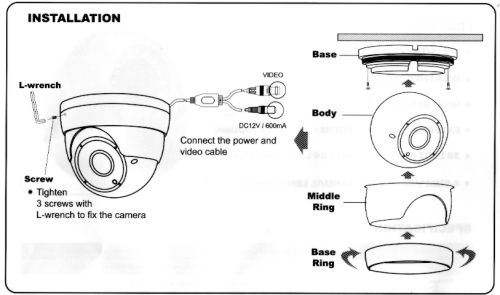
\includegraphics[width=0.60\textwidth]{images/Installation-Diagram}
\end{figure}
\vspace{0.5 in}
\subsection{Camera Operation}
\subsubsection{Scenario}
The camera shall be accessed via secured web interface.
The user shall be required to log on by entering a unique password.
A "live view" from the camera shall be displayed on the user monitor during operation. 
The view shall include pan, tilt, and lens functions (zoom, iris and focus). 
The user shall possess the ability to remotely control all viewing functionality.
The user shall possess the ability to set and clear the movement limits of the pan and tilt mechanisms so equipped.
\subsubsection{Actor(s)}
The use and operation of the camera shall be at the discretion of the administrator and/or user operator.
\vspace{0.5 in}
\begin{figure}[h!]
	\centering
   	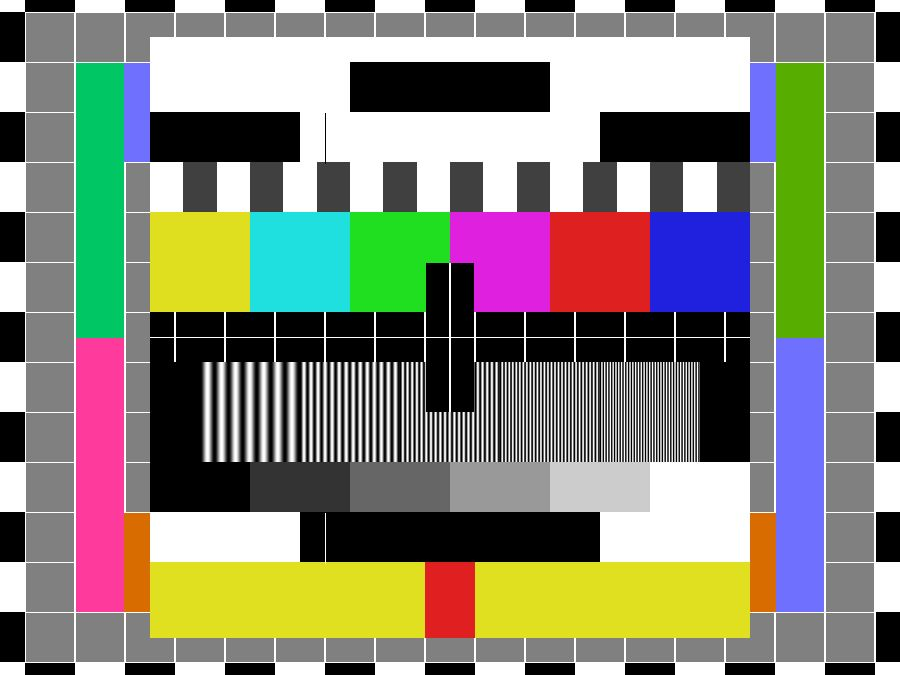
\includegraphics[width=0.60\textwidth]{images/test_image}
\end{figure}
\vspace{0.5 in}
\subsection{Adjusting the Camera}
\subsubsection{Scenario}
The camera shall be adjustable in all features relating to viewing functionality remotely.
The camera shall be adjustable in all features relating to viewing functionality manually on location.
\subsubsection{Actor(s)}
The remote adjusting of all viewing features shall be at the discretion of the administrator and/or user operator.
The manual adjusting of all viewing features shall be the responsibility of only a qualified vendor technician.
\subsection{Routine Maintenance}
\subsubsectio{Scenario}
It is to be advised that routine maintenance be performed both remotely and on location weekly and annually, respectively.
Routine maintenance shall incorporate on location inspections of camera conditions, including the cleanliness of internal systems and the working condition of component connections.
Routine maintenance shall incorporate remote inspections of camera feature functionality, including the pan, tilt, zoom and focusing features.
\subsubsection{Actor(s)}
Routine remote maintenance shall be expected to be performed weekly at the discretion of the administrator and/or user operator.
Routine on location maintenance shall be expected to be performed annually at the discretion of only a qualified vendor technician.
